%*******************************************************
% Capitulo cuatro
%*******************************************************

\chapter{Propuesta metodológica de producción}
\label{capitulometodologia}

El siguiente capítulo describe las dos categorías más fuertes en metodologías de desarrollo de software y realiza un análisis de las caracteristicas que afectan la decisión de escoger una u otra. Al final se plantean alternativas de selección a la metodología y se discute su escenario de aplicación.

\section{Potenciales metodologías de construcción de software}

Se realiza la construcción de una pieza software para el caso de estudio descrito en el capítulo \ref{Caso_de_estudio}. Este caso de estudio tiene las siguientes restricciones, identificadas en el caso de estudio, en su proceso de producción:

\begin{itemize}

    \item La metodología de trabajo empleada por el grupo fue creación coletiva. El proceso ocurre a lo largo de diferentes talleres en los que se hacen actividades de lectura, conversatorios y lluvias de ideas acerca de la muestra. En cada taller se hacen propuestas de trabajo y modificaciones que son valoradas por el grupo. Los requerimientos cambian ante cualquier idea rápidamente aceptada por el grupo.

    \item El proceso debe involucrar una sensibilización acerca de la presencia de la tecnología en el resultado final. El conocimiento de los usuarios de la tecnología se resume en lo tradicional: pantallas, televisores, proyectores y teclados. Todos deben volverse partícipes del proceso de innovación a persar que no tengan conocimientos en tecnología.

    \item Se deben hacer iteraciones frecuentemente. La construcción debe permitir entregas rápidas que le permitan a los miembros del grupo tomar decisiones frente a los construido para evitar reprocesos o que se acepten ideas distantes de lo diseñado previamente.

    \item El fin de los talleres de construcción puede ser otro al de diseñar la obra, por ejemplo describir memorias del pasado o crear piezas físicas para la obra final, por lo que se presenta confusión entre los participantes cuando se les habla de tecnología. Se debe analizar como establecer de forma clara reuniones que funcionen en el marco de alguna metodología que no sea exclusivamente para proyectos de desarrollo de software.

    \item El proceso debe incluir una documentación de contexto para crear un vocabulario común entre los participantes.

\end{itemize}

Toma de decisiones acerca de la producción

Alcance tiempo costo en esta intervención artísticas

Alcance tiempo costo en el caso de estudio

\subsection{Metodologías duras}

Antes de la aparición de las metodologías ágiles dominaban las metodologías que tenían las siguientes características,

\begin{itemize}
  \item Orientación al control del riesgo por iteraciones
  \item Centradas en el diseño
  \item xx
\end{itemize}

La metodología usada en el

Caracteristicas vs creación artística

\subsection{Metodologías ágiles}

Caracteristicas vs creación artística

\section{Selección de la metodología}

Se describe cual adaptación se realiza.










\begin{figure}[h]\label{togafarchimate}
\centering
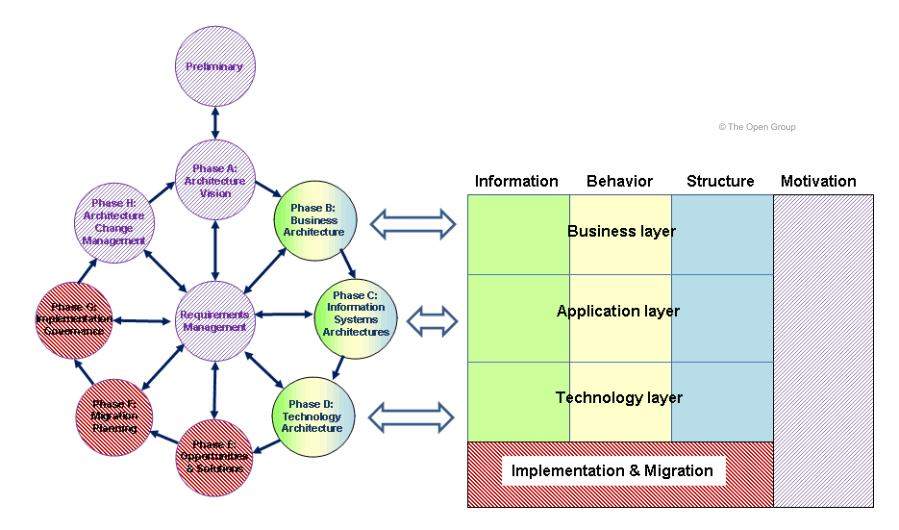
\includegraphics[scale=0.8]{togafarchimate}
\caption{Correspondencia entre Archimate y TOGAF.}
\end{figure}
